\section{PsykologNord - Forretning}
\label{kabitel:Forretning}

Inden vi begynder at se på løsningen, der er blevet lavet i dette projekt, er det nødvendigt at se nærmere på PsykologNord som forretning, og hvad deres problem er.

Først vil vi beskrive PsykologNord som forretning, derefter deres problemstilling, hvem der er påvirket af problemet og en løsning af det.
Dernæst vil flere forskellige løsningsforslag blive betragtet, hvorefter der vil udforskes, hvad den valgte løsning vil give PsykologNord.
Til sidst vil der opstilles nogle målbare krav, som løsningen skal opfylde.

\subsection{Forretningsmodel}
Psykolog Nord er en psykologkæde med 3 afdelinger: en i Aalborg, Aarhus og Odense. De har 3 psykologer:

\begin{itemize}
    \item Katrine Breum Larsen
    \item Miriam Poulsen
    \item Stefan Guldager Boldemann
\end{itemize}

Lige nu er Katrine og Miriam begge tilknyttet afdelingerne i Aalborg og Aarhus, og Stefan er tilknyttet afdelingen i Odense.

Psykolog Nord tilbyder psykologbehandling uden ventetid.
Derfor har de åbent alle 7 dage i ugen fra kl. 9 til 21. De tjener penge på honorarer fra klienter.

De tilknyttede psykologer er ikke ansat af Psykolog Nord, men er partnere.
Derfor skal de ikke betale løn og pension, men derimod har de aftalt, at psykologen modtager halvdelen af betalingen fra klienten.

Firmaet drives af brødrene Anders Mikkelsen og Lasse Kirk, og Lasses kæreste Katrine Breum Larsen.
De har en flad firmastruktur, hvor alle 3 indgår i firmaets ledelse. 
Firmaet tilhører den basale form fra Mintzbergs fem organisationsformer, og på figur \ref{forretning:organisationsdiagram} kan man se deres virksomhedsstruktur.



\subsection{PsykologNords problemstilling}
\label{section:problemstilling}

PsykologNord bruger to informationssystemer til at understøtte deres forretning, se figur \ref{forretning:isfml}.
Dinero bruges som deres regnskabsprogram til at lave og sende fakturaer til deres klienter.

TerapeutBooking er deres nuværende bookingsystem.
Som det kan ses på figur 3 understøttes virksomheden meget af de to informationssystemer, og derfor er det for vigtigt for dem, at de fungerer godt.

PsykologNord har følgende problemer med TerapeutBooking:

\begin{itemize}
    \item TerapeutBooking kan ikke håndtere en bruger tilknyttet flere lokationer.
    Derfor har Katrine to forskellige kalendere: En for hendes klienter i Aarhus og en i Aalborg.
    Det medfører den den konsekvens, at Katrine manuelt skal blokere hendes ene kalender, når hun booker en tid i den anden kalender med en klient. Ellers skal hun bede sekretæren gøre det.
    
    \item TerapeutBooking kan ikke håndtere flere kalendere, der bruger de samme lokaler.
    Det betyder, at da Miriam og Katrine lige nu begge tilbyder samtaler i Aarhus og Aalborg, skal de manuelt gå ind og blokere aftaler i hinandens kalendere.
    Hvis Katrine har en aftale i Aalborg om mandagen klokken 10 til 11, skal hun, eller deres sekretær, blokere tiden i Miriams kalender
    
   \item PsykologNord har, som beskrevet i afsnit \ref{section:forretningsmodel} flere psykologer tilknyttet deres firma.
   Men TerapeutBooking giver ikke en tilfredsstillende måde at styre deres brugeres rettigheder.
   En bruger kan få lov til at ændre alle journaler, se alle journaler eller se ingen journaler.
   På samme måde med fakturaer.
\end{itemize}

De første to problemstillinger betyder, at noget så simpelt som at lave en aftale med en klient går hen og bliver en tidskrævende proces, hvor der også nemt kan ske fejl, se figur \ref{forretning:bpmnnow}.
I følge Katrine bruger sekretæren, Jean, lige nu 1 time om ugen på bare at håndtere bestillinger af aftaler.
Den tredje problemstilling gør, at de ikke kan udvide mere uden, at det kommer til at drukne i et bureaukratisk mareridt i følge dem selv.
Under vores møder med PsykologNord har de givet udtryk for ønsker om at udvide, og bruge lokalerne til et nyt start-up projekt, når de ikke bliver brugt af PsykologNord.
Det vil blive et stort sikkerhedsproblem, hvis flere forskellige firmaer har direkte adgang til hinandens kunder og deres fortrolige oplysninger.



\begin{figure}[H]
    \caption{Informationssystemers understøttelse af FML}
    \centering
        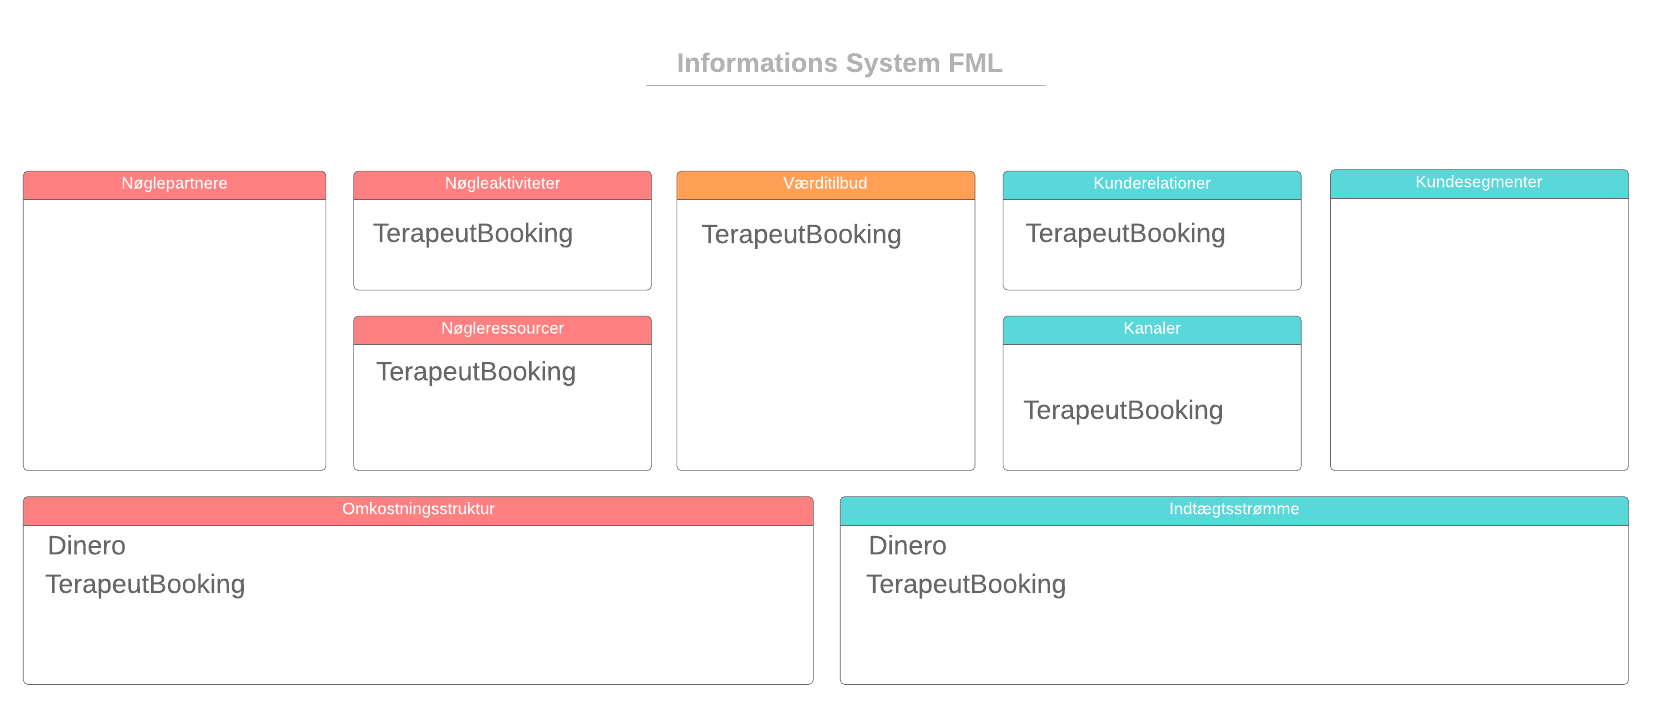
\includegraphics[width=\textwidth]{ISFML.png}
    \label{forretning:isfml}
\end{figure}

\begin{figure}
    \caption{BPMN diagram over at aftale en tid med en klient}
    \centering
        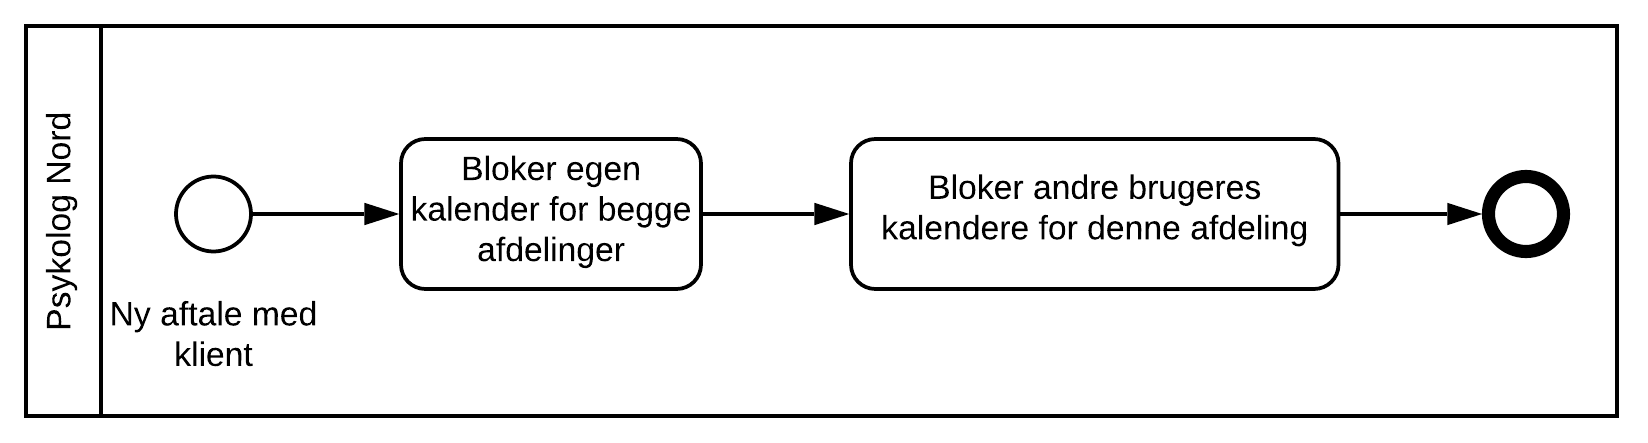
\includegraphics[width=\textwidth]{BPMNNow.png}
    \label{forretning:bpmnnow}
\end{figure}

\subsection{Interessent analyse}

De tre ansatte i Psykolog Nord har en interesse i vores projekt. Vi anser dog ikke alle 3 som primærinteressenter, da Stefan ikke bliver ramt af alle problemerne.
Da Stefan er alene om Odense klinikken oplever han heller ikke de problemer, der bliver nævnt i afsnit \ref{section:problemstilling}.

Lasse Kirk, nævnt i afsnit \ref{section:forretningsmodel}, har også en interesse i projektet, da han og Katrine har udtrykt interesse i at bruge PsykologNords lokaler til et andet firma, når de ikke bliver brugt til samtaler.
Som nævnt i afsnit \ref{section:problemstilling} understøtter deres nuværende løsning ikke booking af det samme lokale på en hensigtsmæssig måde.

Katrine Breum Larsen er chefpsykologen og den primære beslutningstager i samarbejde med Lasse.
Derfor betragtes Katrine og Lasse som primærinteressenterne.

Primærinteressenterne er alle under 35 år, og er derfor ganske habile til brug af computere i deres hverdage.

Miriam og Stefan har også en interesse i projektet, men da de ikke er en del af ledelsen har de ikke en stor indflydelse på projektets udformning.

De betragtes som gidsler ud fra Skriver et al. bog Organisation \cite[s. 435]{interessentanalyse}, da vi har valgt ikke at indblande dem i udviklingsprocessen.
Dette har vi valgt at gøre, da de, som nævnt i afsnit \ref{section:forretningsmodel}, ikke er direkte ansatte i firmaet, men derimod blot partnere.
Desuden har de ikke noget interesse i de andre formål, som Katrine og Lasse vil bruge projektet til. 
Stefans største interesse vil være, at hans hverdag forbliver uændret.

Miriams interesse er at få en nemmere hverdag i forbindelse med bookning af aftaler uden den store omstilling.

PsykologNords klienter er også gidsler, da deres interesse vil være, at deres hverdag forbliver så uændret som muligt, og vi ikke mener, at det vil være en gavn at involvere dem i projektet.

\subsection{Løsningsscenarier}

\subsection{Hvad vil Semplito give PsykologNord?}
Dette afsnit vil beskrive, hvad formålet med projektet er, hvad PsykologNord vil få ud af det, og hvordan vi vil sikre gevinsterne.

\subsubsection{Formål}
Formålet med projektet er:

\begin{itemize}
    \item At forbedre booking processen, så når en klient laver en aftale med en psykolog i et lokale, kan en anden psykolog ikke lave en aftale på samme tidspunkt i samme lokale, uden at psykologen manuelt skal ind og blokere for booking af lokalet.
    \item At forbedre booking processen, så når en klient laver en aftale med en psykolog i en afdeling, kan en anden klient ikke lave en aftale med samme psykolog i en anden afdeling på samme tidspunkt, uden at psykologen manuelt skal melde sig optaget.
    \item At forbedre kundesikkerheden ved at sikre, at en psykolog kun har adgang til sine egne klienters journaler.
\end{itemize}

Hvis man ser på deres forretningsmodellærred, figur \ref{forretning:fml}, vil de første 2 formål gå ind og understøtte deres indtægtsstrømme, nøgleaktiviteter og værditilbud, da det vil give mere tid for Miriam og Katrine, hvor de kan tilbyde behandling.
\subsubsection{Forretningsmæssig løsningsbeskrivelse}

Projektet skal sikre, at PsykologNords bookingproces kommer til at foregå uden, at de manuelt skal ind og rette i hinandens kalendere.
Derudover skal det sikre, at deres psykologer kun kan se deres egne klienters journaler. 
Til sidst skal det også give mulighed for at lave brugere af systemet med andre rettigheder, såsom til deres sekretær, der vil kunne se alle klienter og deres fakturaer, men ikke kunne se nogen klientjournaler.

Til at starte med skal løsningen bruges af PsykologNord, men på længere sigt skal løsningen også bruges af deres andre firmaer.

De ønsker at tage løsningen i brug hurtigst muligt.

\subsubsection{IT-mæssig løsningsbeskrivelse}

PsykologNord vil i fremtiden gerne have bookingsystemet til at være en hjemmeside, men det er på nuværende tidspunkt uden for projektgruppens pensum.
Derfor er de gået med til, at det bliver udviklet som en WPF applikation i .Net C\#, hvor applikationen skal kunne køre på flere computere i et netværk.

PsykologNord har også mange forslag til videreudvikling af systemet, som vi ved, at vi ikke vil kunne nå inden for tidsrammen af projektet.
Derfor er det vigtigt, at løsningen er objektorienteret, så den er nem at videreudvikle på et senere tidspunkt.
Da vi også nu ved, at de senere vil have det som en hjemmeside i stedet for en applikation, skal løsningen også være lagdelt, så blandt andet brugergrænsefladen nemt kan udskiftes.

\subsubsection{Effekter af projektet}
\paragraph*{Økonomiske effekter}
\subparagraph*{Forretningsmæssige investeringer}

Da løsningen skal ind og erstatte en allerede eksisterende løsning skal der stræbes efter, at der ikke bliver den store omvæltning for PsykologNord.

\subparagraph{IT investeringer}

\textit{Interne ressourcer:} PsykologNord skal bruge tid på møder med projektgruppen. Der skal også bruges tid på at svare på spørgsmål over mail og telefon.

\textit{Eksterne ressourcer:} Projektgruppen har startet projektet, men vi har ikke nået at færdiggøre løsningen med alle ønskerne PsykologNord har.
Derfor vil der bagefter skulle hyres softwareudviklere til at videreudvikle på løsningen.

Der skal ikke investeres i hardware, da deres nuværende løsning allerede er digital. Derfor er den totale udgift prisen på at få færdig udviklet løsningen.

\subparagraph{Økonomiske gevinster}

\textit{Forretningsmæssige gevinster:} Det forventes, at den gennemsnitlige tid på at booke en aftale vil blive mindsket.
Der vil også blive en større sikkerhed for klienterne, da alle brugere af systemet ikke vil have adgang til alle klienters oplysninger, og risikoen for bøder pga. datasikkerhed vil blive mindsket.

I det første år eller 2 vil projektet være en udgift, men effektiviseringen af bookingprocessen vil resultere i en besparelse på længere sigt.

\subsubsection{Risikovurdering}
Risikovurderingerne beskrevet i dette afsnit vil sammenligne sikkerhed ved den nuværende løsning og den løsning vi har udviklet i projektet.

\paragraph*{Læk af følsomme personoplysninger}

\subparagraph{Risikovurdering:}
Høj pga. økonomiske konsekvenser og tab af troværdighed ved kunden.
    
\subparagraph{Eksisterende sikring:}
Den nuværende løsning lever op  til alle krav fra Datatilsynet mht. til behandling af følsomme personoplysninger, blandt andet ved at have en krypteret hjemmside.\cite{terapeutbookingsikkerhed}
    
\subparagraph{Handlingsplan:}
Den nye løsning skal også leve op til reglerne fra Datatilsynet. Derudover vil den forbedre sikkerheden ved at begrænse brugernes adgang til klienter i systemet, så en bruger kun har adgang til sine egne klienter.
    
Hvis der skulle ske en læk af data vil PsykologNord følge lovgivningen ved at give Datatilsynet besked, inden for 24 timer efter lækken opdages, og derefter give de involverede klienter besked. Derefter vil lækken lukkes hurtigst muligt.
    
\paragraph*{Tab af klienters fortrolige oplysninger som følge af servernedbrud}

\subparagraph{Risikovurdering:}
Lav
    
\subparagraph{Eksisterende sikring:}
Den nuværende serverløsning har en gennemsnitlig oppetid på 99.5\%. De har 2 separate strømtilslutning, hvilket sikrer deres kørsel mod strømsvigt. Der tages backup af data dagligt, der gemmes i 7 til 30 dage, hvorefter det overskrives. Deres servere er sikret med firewalls og antivirus software, og deres netværksinfrastruktur er optimeret til at kunne modstå alle former for hackerangreb.\cite{terapeutbookingdata}

\subparagraph{Handlingsplan:}
Den nuværende sikring er tilstrækkelig, og derfor er det vigtigt at den nye løsning opfylder samme krav, når den bliver implementeret i virksomheden.

\subsubsection{Gevinster}
\textit{Interne serviceforbedringer:}
Det vil blive nemmere for brugerne af bookingsystemet, når de ikke skal til at lave dobbeltarbejde ved alle aftalerne.

\textit{Risici:}
De største risici med udviklingen af dette projekt er, at vi ikke når langt nok til, at det bliver en erstatning for deres nuværende løsning, og at den nye løsning ikke behandler klienternes fortrolige personoplysninger sikkert nok.
Derfor er det vigtigt, at vi laver et system, der er så nemt som muligt at videreudvikle på, og at det er sikkert nok til, at uvedkommende ikke bare kan få adgang til fortrolige personoplysninger.

\subsubsection{Implementering og Opfølgning}

For at sikre, at den udarbejdede løsning er en forbedring af deres nuværende system, er der blevet opstillet følgende key performance indicators(KPI'er):

\begin{table}[H]
\begin{tabular}{|l|l|}
\hline
KPI:                                                                                                       & Antal timer sparet på booking                                                                                                                    \\ \hline
Hvorfor måles?                                                                                             & \begin{tabular}[c]{@{}l@{}}Booking procesen er lige nu tidskrævende,\\ og vi vil derfor gerne kunne se om\\ vores løsning er bedre.\end{tabular} \\ \hline
Hvordan måles?                                                                                             & Det kan måles med et stopur.                                                                                                                     \\ \hline
\begin{tabular}[c]{@{}l@{}}Hvem er ansvarlig\\ for måling?\end{tabular}                                    & Chefpsykolog Katrine Breum Larsen                                                                                                                \\ \hline
Forventet målingsdato                                                                                      & Hver gang der foretages en booking.                                                                                                              \\ \hline
\begin{tabular}[c]{@{}l@{}}Forventet værdiinterval\\ for måling\end{tabular}                               & 5-10 minutter                                                                                                                                    \\ \hline
Måling                                                                                                     & Endnu ikke udført                                                                                                                                \\ \hline
\begin{tabular}[c]{@{}l@{}}Handlingsplan i fald måling\\ falder uden for forventet\\ interval\end{tabular} & \begin{tabular}[c]{@{}l@{}}Opdatere programmet så det vil være mere\\ effektivt end den nuværende løsning.\end{tabular}                          \\ \hline
Ansvarlig for handling                                                                                     & Katrine Breum Larsen                                                                                                                             \\ \hline
\end{tabular}
\end{table}

\begin{table}[H]
\begin{tabular}{|l|l|}
\hline
KPI:                                                                                                       & Antal timer brugt på rettelser af booking                                                                                                                                                \\ \hline
Hvorfor måles?                                                                                             & \begin{tabular}[c]{@{}l@{}}Rettelsesprocessen i den nuværende\\ løsning er meget tidskrævende. Derfor\\ er det vigtigt for os at se, om den nye\\ løsning er mere effektiv.\end{tabular} \\ \hline
Hvordan måles?                                                                                             & Det kan måles med et stopur.                                                                                                                                                             \\ \hline
\begin{tabular}[c]{@{}l@{}}Hvem er ansvarlig\\ for måling?\end{tabular}                                    & Chefpsykolog Katrine Breum Larsen                                                                                                                                                        \\ \hline
Forventet målingsdato                                                                                      & Hver gang der foretages en booking.                                                                                                                                                      \\ \hline
\begin{tabular}[c]{@{}l@{}}Forventet værdiinterval\\ for måling\end{tabular}                               & 5-10 minutter                                                                                                                                                                            \\ \hline
Måling                                                                                                     & Endnu ikke udført                                                                                                                                                                        \\ \hline
\begin{tabular}[c]{@{}l@{}}Handlingsplan i fald måling\\ falder uden for forventet\\ interval\end{tabular} & \begin{tabular}[c]{@{}l@{}}Opdatere programmet så det vil være mere\\ effektivt end den nuværende løsning.\end{tabular}                                                                  \\ \hline
Ansvarlig for handling                                                                                     & Katrine Breum Larsen                                                                                                                                                                     \\ \hline
\end{tabular}
\end{table}

\begin{table}[H]
\begin{tabular}{|l|l|}
\hline
KPI                                                                                                        & \begin{tabular}[c]{@{}l@{}}Antal gange tilgået anden psykologs\\ patients journal.\end{tabular}                        \\ \hline
Hvorfor måles?                                                                                             & \begin{tabular}[c]{@{}l@{}}For at sikre, at der ikke sker\\ sikkerhedsbrud, samt for at\\ overholde GDPR.\end{tabular} \\ \hline
Hvordan måles?                                                                                             & Måles med en tæller                                                                                                    \\ \hline
\begin{tabular}[c]{@{}l@{}}Hvem er ansvarlig\\ for måling?\end{tabular}                                    & Chefpsykolog Katrine Breum Larsen                                                                                      \\ \hline
Forventet målingsdato?                                                                                     & \begin{tabular}[c]{@{}l@{}}Ugentligt det første kvartal efter systemets\\ implementeret.\end{tabular}                  \\ \hline
\begin{tabular}[c]{@{}l@{}}Forventet værdiinterval\\ for måling\end{tabular}                               & 0                                                                                                                      \\ \hline
Måling                                                                                                     & Ikke udført                                                                                                            \\ \hline
\begin{tabular}[c]{@{}l@{}}Handlingsplan i fald måling\\ falder uden for forventet\\ interval\end{tabular} & \begin{tabular}[c]{@{}l@{}}Opdatere programmet, så det bliver mere \\ sikkert.\end{tabular}                            \\ \hline
Ansvarlig for handling                                                                                     & Katrine Breum Larsen                                                                                                   \\ \hline
\end{tabular}
\end{table}
